\documentclass[12pt,onecolumn,a4paper,fleqn]{article}
\usepackage[top=1in, bottom=1in, left=0.75in, right=0.75in]{geometry}
\usepackage{epsfig,graphicx,subfigure,amsthm,amsmath}
\usepackage[table,xcdraw,svgnames]{xcolor}
\usepackage{setspace}
\usepackage{mathtools}
\usepackage{fancyhdr}
\usepackage{sidecap}
\usepackage{tikz}
\usepackage{pgfplots}
\usetikzlibrary{decorations.pathreplacing}
\usepackage{relsize}
\usepackage{color,xcolor}
\usepackage[framed,numbered]{matlab-prettifier}
\usepackage{float}
\usepackage{enumerate}
\usepackage{booktabs}
\usepackage{setspace}
\usepackage{datetime}
\usepackage{xepersian}


\settextfont[Path=fonts/,BoldFont={ZarBd.ttf},BoldFeatures={Scale=0.9}]{BZar.ttf}

%\DeclarePairedDelimiter\ceil{\lceil}{\rceil}
%\DeclarePairedDelimiter\floor{\lfloor}{\rfloor}

\definecolor{vgreen}{RGB}{104,180,104}
\definecolor{vblue}{RGB}{49,49,255}
\definecolor{vorange}{RGB}{255,143,102}

\pagestyle{fancy}
\fancyhf{}
\rhead{\textbf{آزمایشگاه طراحی سیستم‌های دیجیتال}}
\chead{\textbf{گزارش آزمایش دوم}}
\lhead{\textbf{\nouppercase{\rightmark}}}
\cfoot{({\thepage})}
\renewcommand{\headrulewidth}{1pt}
\renewcommand{\footrulewidth}{1pt}
\renewcommand{\sectionmark}[1]{\markright{#1}}
\renewcommand{\subsectionmark}[1]{\markright{#1}}
%\newdateformat{monthyeardate}{%
%	\monthname[\THEMONTH], \THEYEAR}

\onehalfspacing
\begin{document}
	%%% title pages
	\large
	\begin{titlepage}
		
		\begin{center}
			\begin{huge}
				\textbf{
					به نام خدا\\
				}
			\end{huge}
			
			\vspace*{1.5cm}
			
\includegraphics[scale=0.9]{source/sharif_logo.png}\\
			\vspace*{0.5cm}
			\begin{Large}
				
					دانشگاه صنعتی شریف\\
					\vspace*{0.25cm}
				\textbf{
					دانشکده مهندسی کامپیوتر\\
				}
			\end{Large}
			\vspace*{3cm}
			\begin{huge}
				\textbf{
					آزمایشگاه طراحی سیستم‌های دیجیتال\\
					\vspace*{1.75cm}
				}
			\end{huge}
			
			\begin{Large}
				\textbf{
					آزمایش دوم:\\
					طراحی شماتیک مدار ترتیبی\\
				}
			\end{Large}
			
			\noindent\rule[1ex]{\linewidth}{1pt}
			\vspace*{1.5cm}
			\begin{Large}
				محمدجواد هزاره، یاسین موسوی
				
				\vspace*{1.5cm}
				%					\textbf{\today}
				\textbf{
					تابستان 1400
				}
			\end{Large}			
		\end{center}
		\thispagestyle{empty}
	\end{titlepage}	
	\pagebreak
	
	\tableofcontents
	\thispagestyle{empty}
	\pagebreak
	\section{مقدمه}
	\subsection{هدف آزمایش}
	هدف از این آزمایش آشنایی با ابزار طراحی به کمک شماتیک و طراحی یک مدار ترتیبی است.
	\subsection{شرح آزمایش}
	در این آزمایش می‌خواهیم یک سیستم کنترل‌کننده اتومات در طراحی کنیم. هدف، کنترل کردن بازکردن درِ ورودی و بستن درِ خروجی است. اتاق ظرفیت ۱۵ نفره دارد و بنابراین اگر تعداد افراد حاضر در اتاق ۱۵ نفر باشد نباید در باز شود. هم‌چنین برای ورود بازه زمانی مشخصی فرصت داریم و در خارج از این بازه نیز نباید درِِ ورودی را باز کنیم.
	درِ خروجی اما مادامی که حداقل یک نفر در اتاق وجود دارد باز است و درصورتی که اتاق خالی شود بسته می‌شود.
	\pagebreak
	\section{توصیف معماری سیستم}
	\subsection{رابط کاربری سیستم}
	مطابق شکل \ref{fig:interface}، مدار شامل ۶ ورودی است که دو وردی
	\lr{IN}
	و
	\lr{OUT}
	به ترتیب زمانی ۱ می‌شوند که فردی به پشت در ورودی رسیده، و از در خروجی عبور کند. سیگنال
	\lr{Ent}
	نیز زمانی ۱ می‌شود که فردی که قصد ورود دارد، دکمه ورود را فشار دهد. سیگنال
	\lr{T}
	نیز از سیستم ساعت می‌آید، و اگر ۱ باشد یعنی در بازه زمانی مناسب برای ورود هستیم و در غیر این‌صورت یعنی زمان ورود گذشته یا هنوز آغاز نشده است. سیگنال‌های 
	\lr{clk}
	و
	\lr{clear}
	نیز به ترتیب کلاک مدار و سیگنال ری‌ست کردن شمارنده موجود در مدار هستند.
	
	\begin{figure}[H]
		\centering
		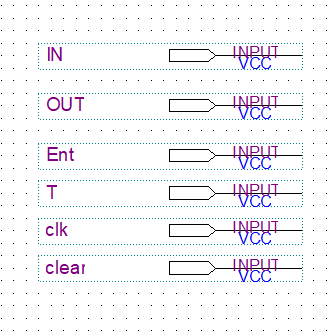
\includegraphics[scale=0.8]{source/interface.png}
		\caption{ورودی‌های مدار}
		\label{fig:interface}
	\end{figure}
	خروجی‌های مدار نیز شامل دو سیگنال 
	\lr{open}
	و
	\lr{close}
	اولی اگر ۱ باشد درِ ورودی باز می‌شود و در غیر این‌صورت بسته. دومی نیز اگر ۱ باشد درِ خروجی بسته می‌شود و در غیر این‌صورت باز.
	\subsection{نحوه کار مدار}
	برای پیاده‌سازی مدار، از یک شمارنده ۴-بیتی استفاده شده است که تعداد افراد حاضر در اتاق را می‌شمارد و در هر مرحله با توجه به این‌که کسی خارج شده و یا قصد ورود دارد و در باز شده است یا خیر، این شمارنده یکی زیاد و یا یکی کم می‌شود.
	
	و اما ورود و خروج افراد به اتاق چهار حالت زیر را داراست:
	\begin{itemize}
		\item (00): 
		نه کسی قصد ورود داشته و نه کسی خارج شده باشد. در این‌صورت شمارنده را غیرفعال می‌کنیم که همان وضعیت قبلی خود را نگه‌دارد. مشخصا سینگال خروجی
		\lr{open}
		نیز مقدار صفر خواهد داشت و درِ ورودی بسته خواهد ماند.
		\item (01):
		کسی قصد ورود ندارد، اما یک نفر از اتاق خارج شده. در این حالت شمارنده را فعال کرده و نحوه شمارش آن را به صورت رو به پایین انتخاب می‌کنیم تا یکی کم شود.
		\item (10):
		یک نفر قصد ورود دارد، اما کسی خارج نشده است. در این حالت نخست چک می‌کنیم که فرد دکمه ورود را فشرده باشد و سپس اگر تعداد افراد کمتر از ۱۵ نفر بود و در بازه زمانی مناسب برای ورود بودیم، سیگنال خروجی
		\lr{open}
		را ۱ کرده و هم‌چنین شمارنده را فعال می‌کنیم و آن را به صورت شمارش رو به بالا قرار می‌دهیم تا یکی به تعداد بیافزاید.
		\item (11):
		یک نفر قصد ورود دارد و هم‌زمان یک نفر نیز خارج شده است. در این حالت شمارنده را غیر فعال می‌کنیم تا تعداد تغییری نکند و فقط سیگنال خروجی
		\lr{open}
		را ۱ می‌کنیم.
	\end{itemize}
	برای سیگنال خروجی
	\lr{close}
	نیز فقط از عدد خروجی شمارنده استفاده می‌کنیم و هرگاه این عدد صفر شد، این سیگنال را نیز فعال می‌کنیم و در غیر این‌صورت صفر نگه می‌داریم.
	\begin{figure}[H]
		\centering
		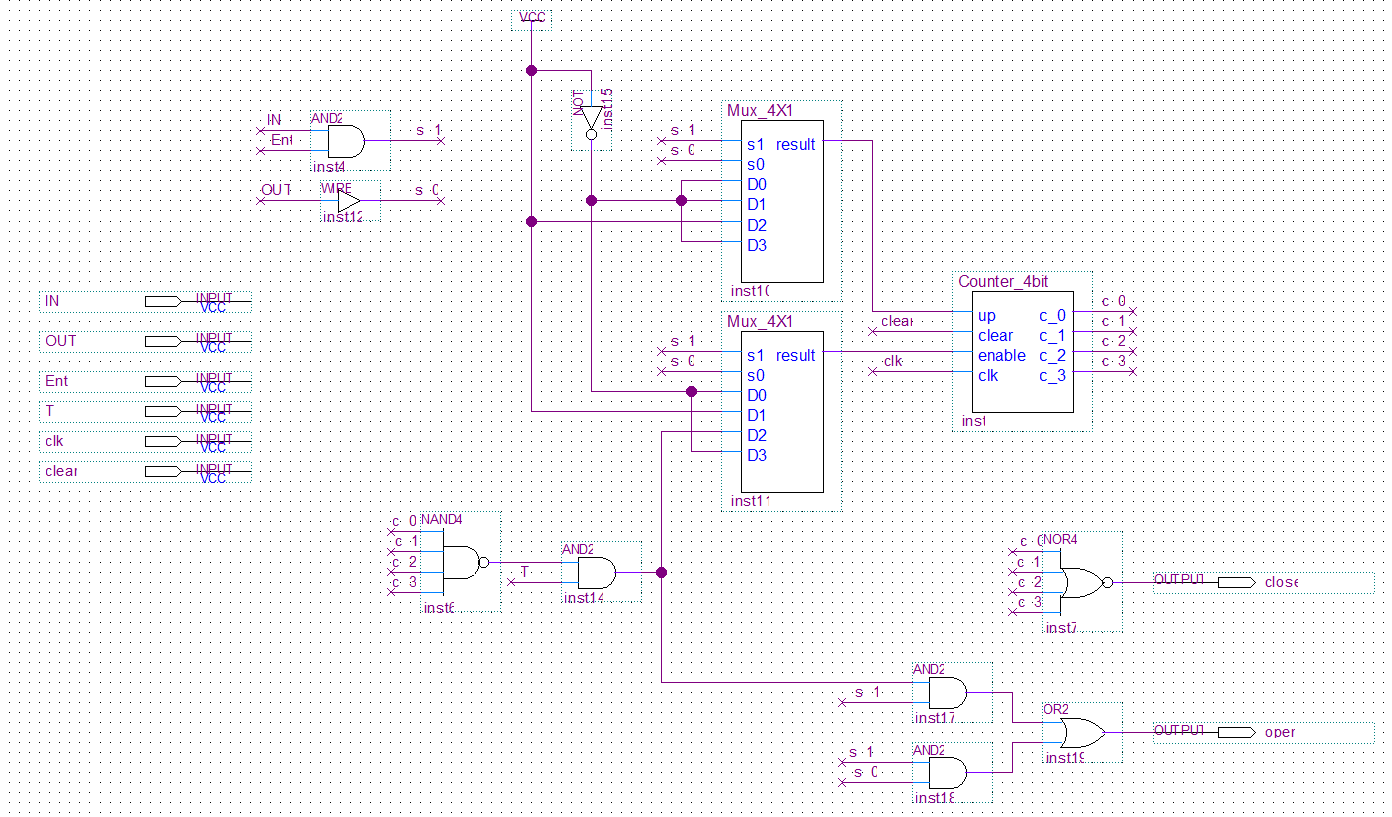
\includegraphics[scale=0.6]{source/circuit.png}
		\caption{نمای کلی مدار}
		\label{fig:circuit}
	\end{figure}

	\subsection{توصیف ماژول‌ها}
	\subsubsection{شمارنده ۴-بیتی}
	این ماژول یک شمارنده ۴-بیتی است که در هر دو جهت رو به بالا و پایین می‌شمارد. مدار داخلی این ماژول را می‌توانید در شکل \ref{fig:counter} مشاهده کنید.
	\begin{figure}[H]
		\centering
		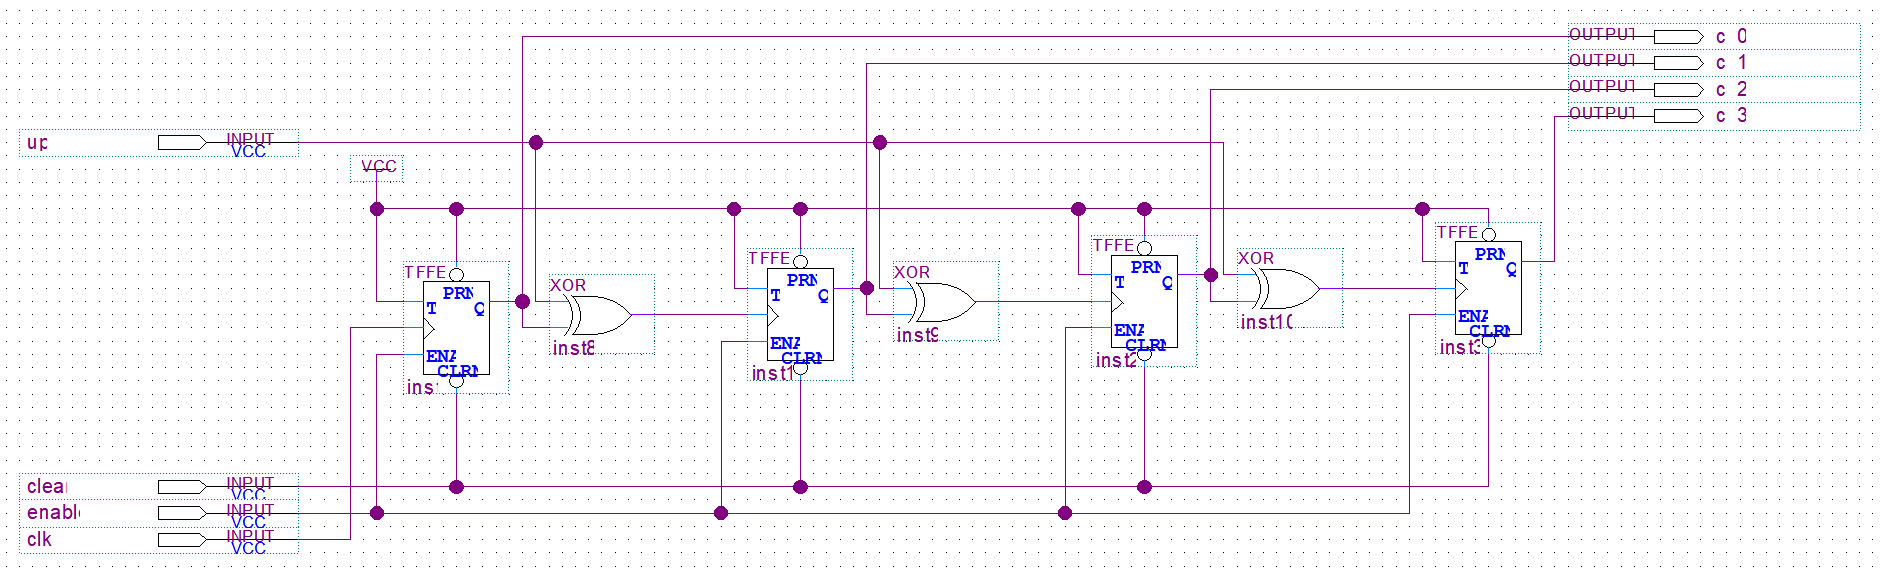
\includegraphics[scale=0.4]{source/counter.png}
		\caption{طراحی داخلی ماژول شمارنده}
		\label{fig:counter}
	\end{figure}
 	
 	\pagebreak
 	\section{شبیه‌سازی}
 	شکل موج حاصل از شبیه‌سازی مدار نیز در شکل \ref{fig:simulation} نشان داده شده است.
 	\begin{figure}[H]
 		\centering
 		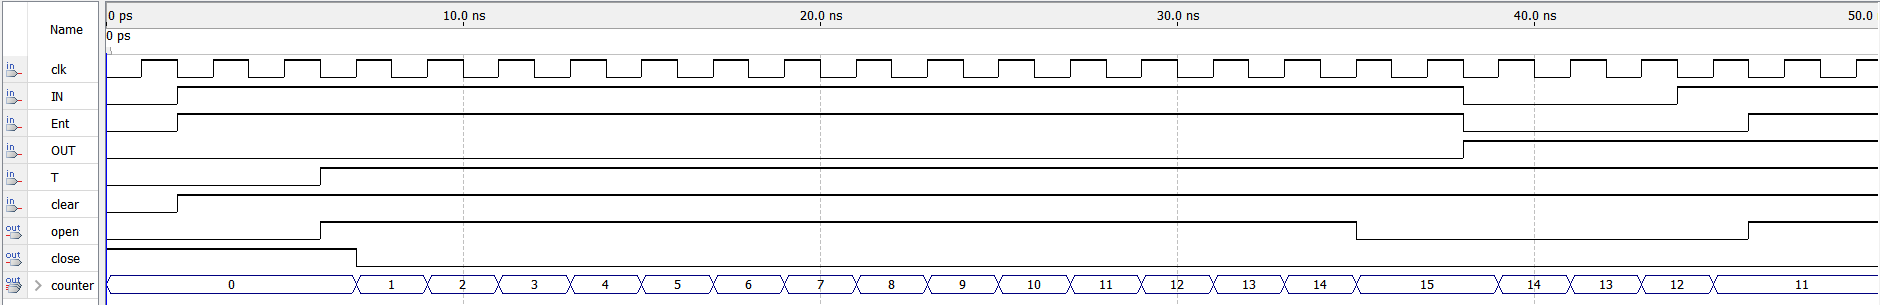
\includegraphics[scale=0.43]{source/simulation.png}
 		\caption{شکل موج}
 		\label{fig:simulation}
 	\end{figure}
 	
\end{document}